\documentclass[12pt]{article}
\usepackage[margin=1in]{geometry}
\usepackage[utf8]{inputenc}
\usepackage{graphicx} % for \includegraphics
\usepackage{listings} % for formatting code
\usepackage{hyperref} % for autoref
\usepackage{amsmath}  % for \begin{cases}
\usepackage{float}    % for positioning figures
\usepackage{xcolor}   % for properly coloring links
\usepackage[all]{hypcap} % for linking to the top of figures rather than captions
\usepackage{color}
\usepackage{caption}

\lstset{basicstyle = \ttfamily,columns=fullflexible}

\graphicspath{ {images/} }

\usepackage{color} %red, green, blue, yellow, cyan, magenta, black, white
\definecolor{mygreen}{RGB}{28,172,0} % color values Red, Green, Blue
\definecolor{mylilas}{RGB}{170,55,241}

\newcommand*{\captionsource}[2]{%
  \caption[{#1}]{%
    #1%
    \\\hspace{\linewidth}%
    \textbf{Source:} #2%
  }%
}

\hypersetup{
    colorlinks,
    linkcolor= black,
    citecolor={blue!50!black},
    urlcolor={blue!80!black}
}

\lstset{language=[x86masm]Assembler,%
    %basicstyle=\color{red},
    breaklines=true,%
    morekeywords={matlab2tikz},
    keywordstyle=\color{blue},%
    morekeywords=[2]{1}, keywordstyle=[2]{\color{black}},
    identifierstyle=\color{black},%
    stringstyle=\color{mylilas},
    commentstyle=\color{mygreen},%
    showstringspaces=false,%without this there will be a symbol in the places where there is a space
    numbers=left,%
    numberstyle={\tiny \color{black}},% size of the numbers
    numbersep=9pt, % this defines how far the numbers are from the text
    emph=[1]{for,end,break},emphstyle=[1]\color{red}, %some words to emphasise
    %emph=[2]{word1,word2}, emphstyle=[2]{style},    
}

\newcounter{nalg}[chapter] % defines algorithm counter for chapter-level
\renewcommand{\thenalg}{\thechapter \arabic{nalg}} %defines appearance of the algorithm counter
\DeclareCaptionLabelFormat{algocaption}{Algorithm \thenalg} % defines a new caption label as Algorithm x.y

\lstnewenvironment{algorithm}[1][] %defines the algorithm listing environment
{   
    \refstepcounter{nalg} %increments algorithm number
    \captionsetup{labelformat=algocaption,labelsep=colon} %defines the caption setup for: it ises label format as the declared caption label above and makes label and caption text to be separated by a ':'
    \lstset{ %this is the stype
        mathescape=true,
        frame=tB,
        numbers=left, 
        numberstyle=\tiny,
        basicstyle=\scriptsize, 
        keywordstyle=\color{black}\bfseries\em,
        keywords={,input, output, return, datatype, function, in, if, else, foreach, while, begin, end, } %add the keywords you want, or load a language as Rubens explains in his comment above.
        numbers=left,
        xleftmargin=.04\textwidth,
        #1 % this is to add specific settings to an usage of this environment (for instnce, the caption and referable label)
    }
}
{}

\title{
    An Implementation of Fault Tolerant Computing Techniques\\
}
\author{
    David Knight\\
}
\date{Dec 15, 2021}

\begin{document}

\maketitle

\begin{center}

\tableofcontents

\end{center}

\pagebreak

\section{Proposal}
This project will implement two methods of fault tolerant computing by modifying a single cycle MIPS processor. A MIPS processor will be modified to become a lockstep processor similar to an ARM Cortex R processor such that a second core is running the same program but delayed by 1 clock cycle. The ALU of the MIPS processor will be modified using a technique called Triple Modular Redundancy (TMR) such that any errors during computation will not detected and fixed. The TMR will operate seamlessly to the program that is being run however an error detected by the lockstep CPU will cause a system reset. The MIPS processor will only support a few simple instructions such as simple ALU operations and load/store instructions; branch and jump instructions will not be supported so the design can be completed in a reasonable time.

The project will be implemented in VHDL using the Vivado simulator. The processor instruction memory and data memory will be initialized with two separate memory files at startup. Modules such as the ALU and the register file will be implemented with generics which introduce bit flips to logic to create momentary "faults" which will cause errors in computation. Through simulation both the TMR and the lockstep processor modifications will be show to either detect or even correct these errors.

The base single cycle MIPS processor will be implemented by 15th of November. TMR will be implemented in the ALU by the 22th of November. The complete lockstep CPU will be implemented by the 8th of December. The final report will be completed by the 15th of December

List of deliverables:
\begin{itemize}
    \item Final project report.
    \item VHDL code implementing features described above.
    \item Example program to be run on the processor (Including Assembly and machine code implementations).
    \item Initialization file for RAM.
\end{itemize}

\section{MIPS Design}
This processor is a simple design that implements the basic architecture of a single cycle MIPS processor including the fetch, decode, execute, memory access and write back stages. The instruction memory is initialized on reset with a hard coded program, the program is show below in listing \ref{lst:program}. This program tests the load instruction and a number of basic ALU instructions. The store instruction is not tested because it will not demonstrate anything that the load instruction cannot show.

\lstinputlisting[numbers=none, label={lst:program}, caption={Example program run on processor.}, keepspaces]{program.asm}

The data memory is also initialized on reset with the value $0x0D$ in R0 and $0x1D$ in R1. After the program is successfully executed registers R2-R7 should contain the values 0x0D, 0x1D, 0x10, 0x2A, 0x10, and 0x179 respectively. See \autoref{fig:successOutput} for a simulation of the result of the program when completed successfully.

\begin{figure}[H]
    \centering
    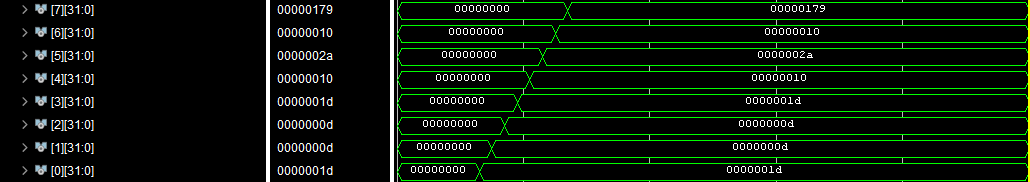
\includegraphics[width=0.7\textwidth]{success.png}
    \caption{Successful output of the program.}
    \label{fig:successOutput}
\end{figure}

\section{Triple Modular Redundancy ALU}
\subsection{Implementation}
In it's most simplest form Triple Modular Redundancy is implemented with 3 copies of the module being tested are instantiated and then all the outputs being fed into a "voter" module that selects the most correct answer. A simple example is shown in \autoref{fig:basic_tmr} where a Boolean logic gate is implemented with TMR. 3 copies of the gate are instantiated and then a majority gate is implemented where the most common gate output is selected as the final answer.

\begin{figure}[H]
    \centering
    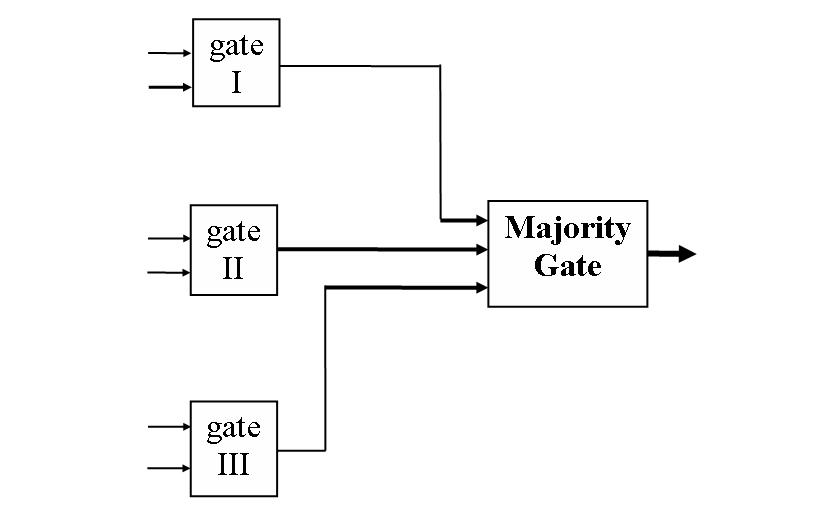
\includegraphics[width=0.7\textwidth]{Triple_Modular_Redundancy.jpg}
    \captionsource{A simplified diagram of TMR.}{https://en.wikipedia.org/wiki/Triple\_modular\_redundancy}
    \label{fig:basic_tmr}
\end{figure}

This example is greatly simplified because each gate can output only one of two options, logic high or logic low, therefor the majority gate will always have at least two gates in agreement. For our ALU design we will instantiate 3 different ALUs however each ALU output will have 32 bits of output that our new majority gate will need to decide between and to make things more difficult we decided to make this TMR design transparent to the user which means that we can't alert the user if all gates disagree.

The compromise I chose to make is to choose ALU0 when the correct answer when all gates disagree. While this is a limitation to the design the logic is greatly simplified because the only case were ALU0 will not be chosen is when ALU1 = ALU2. If ALU1 != ALU2 then either ALU0 will equal ALU1 or ALU2 or neither, in any cause ALU0 is the resulting answer. Because we don't need to report disagreement between all gates no more logic is required to meet the design requirements. Thus the majority gate logic can be simplified to:
\begin{algorithm}[caption={ALU Majority Gate Logic.}, label={majority_gate_logic}]
if (ALU1 = ALU2)
    choose ALU1
else
    choose ALU0
\end{algorithm}

\subsection{Simulation}
To simulate a fault in the ALU I have added a generic which when set to 1 causes the output of the ALU to always be stuck at A5A5A5A5 regardless of inputs or the operation being performed. While most failures would likely be more subtle the TMR operation will be the same. First in \autoref{fig:aluFault} we can see the output of the program when the fault occurs without TMR enabled. Next in \autoref{fig:tmrSuccess} we can see the output of the program when TMR is enabled, notice signal alu\_out[0] is stuck at A5A5A5A5 however alu\_out[1] and alu\_out[2] are correct.

\begin{figure}[H]
    \centering
    \includegraphics[width=0.7\textwidth]{aluFault.PNG}
    \caption{A fault in the ALU causing the outputs to be incorrect.}
    \label{fig:aluFault}
\end{figure}

\begin{figure}[H]
    \centering
    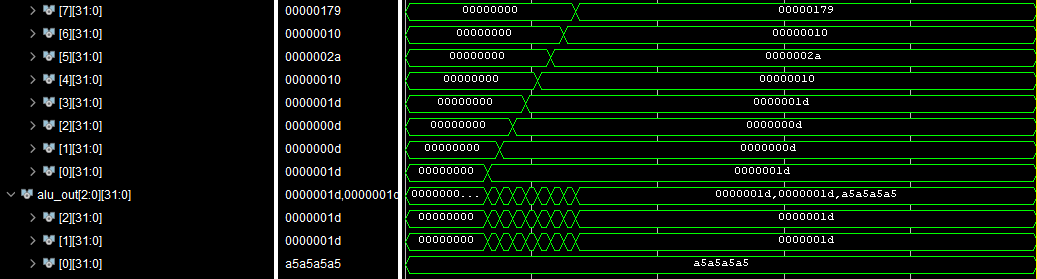
\includegraphics[width=0.7\textwidth]{tmrSuccess.PNG}
    \caption{A fault in the ALU being corrected by TMR.}
    \label{fig:tmrSuccess}
\end{figure}

\section{Lockstep Processor Design}
\subsection{Implementation}
Generally speaking a lockstep system is a system where a second copy of the system is instantiated and run in parallel to the primary system to determine if a fault occurs. A fault is found when one of the two systems disagree with each other in some way. Unlike the TMR design the lockstep design is less standardized which means we have much more freedom both in determining how we determine a fault has occurred and how to respond to it.

For our design I will determine a fault by comparing key signals between the primary and redundant processors. The compared signals will consist of the program counter, outputs of the control unit, and inputs/outputs of the ALU. If any of these signals in the primary processor disagrees with the corresponding signals in the redundant processor a reset signal will be send to both processors to prevent continued execution on faulty hardware.

%All signals that will be compared between the CPUs will be made outputs from the CPU design so they can be compared in a top level module. All compared signals that are just a Boolean can be compared using a simple xor operation a signal that is true when the two processor signals are out of step. Signals that are more than one bit in size can be xor'd together and then all of the resulting bits can be or'd together to get our final out of step signal. Finally all of these out of step signals can be or'd together to create a signal signal that is true when the primary and redundant processors are out of step. This signal can be or'd with the external reset signal to reset both processors.

\subsection{Simulation}
A lockstep fault will be simulated adding a generic to the control unit which will cause the regDst signal to be stuck at logic low on R type instructions when the proper regDst signal should be logic high. regDst is one of the signals tracked by the top level lockstep logic which should catch this fault when it occurs.

\autoref{fig:lockstepSuccess} shows the simulation results when this fault is triggered on the first R type instruction which is located at instruction memory address 0x02. During execution of the R type instruction the lockstep\_regDst[1] signal is properly set to logic high while the lockstep\_regDst[0] signal is incorrectly held at logic low. On the rising edge of the following clock cycle the regDst\_out\_of\_step signal is set to logic high which then causes the out\_of\_step signal to go to logic high. This out\_of\_step signal finally triggers the reset signal which returns both processors back to instruction 0x00.

\begin{figure}[H]
    \centering
    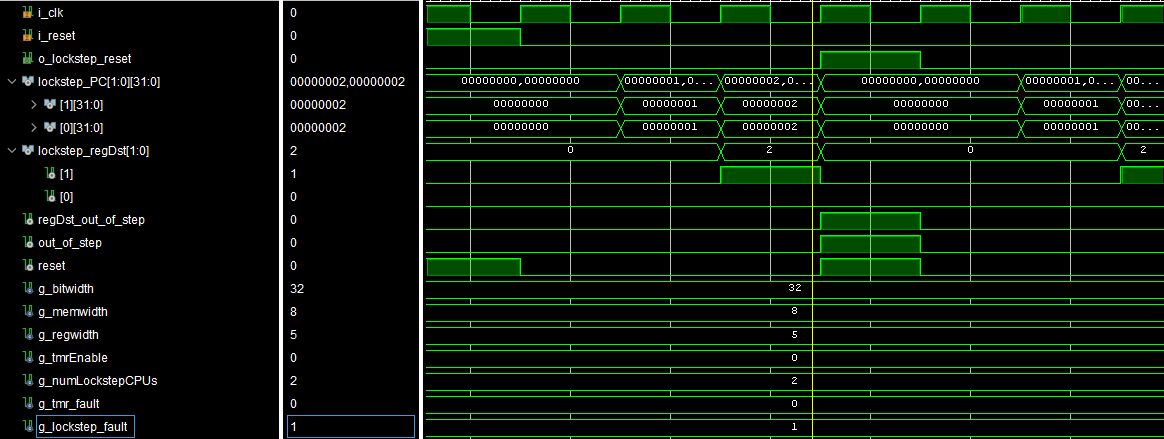
\includegraphics[width=0.7\textwidth]{lockstepSuccess.PNG}
    \caption{A fault in the control unit is detected by the lockstep logic.}
    \label{fig:lockstepSuccess}
\end{figure}

\section{Future Improvements}
Throughout this design I have had to make a number of compromises to make the design practical for a single semester project, however I have had a number of ideas on possible improvements that could improve the function or simulation of the design. Below I have listed some of these future improvements that can be investigated

\begin{itemize}
    \item The lockstep reset signal does not necessarily have to trigger a reset but could instead be used to trigger an interrupt service routine which would allow the user to program in their own response to faults. This functionality would be similar to the lockstep feature in the ARM Cortex-R family of processors.
    
    \item The current design adds physical separation between both CPUs so a simple fault that affects one section of the silicon but not the other will be detected by this feature. However to add more protection we could introduce temporal separation by running the redundant CPU a few clock cycles behind the primary CPU. I thinks this could be implemented by adding FIFOs to all of the input signals of the redundant CPU and FIFOs to all of the outputs signals of the primary CPU. This would keep the lockstep comparisons between the two processors in sync while keeping each CPU a few clock cycles separated.
    
    \item Because the lockstep fault is not a simple transient failure the CPU actually gets caught in a reset loop where the processor is reset every 3 clock cycles. Possible solutions for this problem might include turning the processor off after the lockstep fault has occurred on the same instruction more than once.
    
    \item 
\end{itemize}
Lockstep can be improved by adding temporal separation between the CPUs, a FIFO can be used to delay the CPU signals for comparison.

The lockstep reset signal could be used to trigger and ISR to handle faults rather than triggering resets. This would be similar to the ARM Cortex-R processor.

Because this fault is hard coded into the CPU and not just a transient failure the processor is actually caught into a reset loop whereby the processor is reset every 3 clock cycles.

The primary and redundant lockstep CPUs instantiate their own copies of instruction memory and data memory, a more realistic design would use only a single copy of each to reduce size of the processor and possible implement something like ECC memory on both to find faults there.

Use the alias and force to simplify the testbench. Also make the designs in a for generate loop.

Maybe have the TMR ALU trigger a reset when all 3 ALUs disagree.

\section{Conclusion}


\end{document}
